\documentclass[11pt]{article}

\usepackage[margin=1.1in]{geometry}
\usepackage[utf8]{inputenc}
\usepackage[T1]{fontenc}
\usepackage{lmodern}
\usepackage{microtype}
\usepackage{graphicx}
\usepackage{booktabs}
\usepackage{amsmath}
\usepackage[round]{natbib}
\usepackage[labelsep=period,font=small]{caption}
\usepackage{tikz}
\usetikzlibrary{positioning,arrows.meta}
\usepackage[hidelinks]{hyperref}
\usepackage{xcolor}

\newcommand{\repo}{\url{https://github.com/IshaanAyaan/slm-agents}}

% Auto-generated from run logs by slm_harness/scripts/fill_phase2_paper.py.
% Every number in the results section originates in committed JSON artifacts.
% AUTO-GENERATED by slm_harness/scripts/fill_phase2_paper.py. Do not edit.
\newcommand{\floorSummarySentence}{Of the eight subroutines, 3 clear the bar at or below 500M parameters, 1 of them already at 135M; for 3 the rules baseline alone suffices; 2 remain unsolved at every tested size.}
\newcommand{\minSchemaValidityFTPct}{42}
\newcommand{\schemaValiditySentence}{Fine-tuned schema validity is at least 92 percent in 31 of 32 cells; the lone exception is \texttt{path\_normalizer} at 135M with 42 percent. Base instruct models at the same two smallest sizes collapse to zero schema validity on most subroutines under identical prompts, so format reliability is bought by fine-tuning, not by scale.}
\newcommand{\nTrainPerSub}{2000}
\newcommand{\nValPerSub}{150}
\newcommand{\nTestPerSub}{300}
\newcommand{\nTestEval}{250}
\newcommand{\floorTableBody}{\begin{tabular}{lrrrrrll}
\toprule
Subroutine & Rules & 135M & 362M & 494M & 1544M & Floor & Verdict \\
\midrule
\texttt{action\_router} & 0.277 & 0.612 & 0.740 & \textbf{0.936} & \textbf{0.996} & 494M & works at 494M \\
\texttt{evidence\_judge} & 0.983 & 0.540 & 0.484 & 0.844 & 0.932 & -- & rules suffice \\
\texttt{json\_repair} & 0.147 & \textbf{0.924} & \textbf{1.000} & \textbf{0.996} & \textbf{1.000} & 135M & works at 135M \\
\texttt{path\_normalizer} & 0.790 & 0.500 & 0.704 & \textbf{0.956} & \textbf{0.980} & 494M & works at 494M \\
\texttt{read\_span\_selector} & 0.817 & 0.000 & 0.024 & 0.224 & 0.816 & -- & unsolved (best 0.82 at qwen2.5-1.5b) \\
\texttt{search\_hit\_ranker} & 0.993 & 0.160 & 0.176 & 0.948 & 0.996 & -- & rules suffice \\
\texttt{search\_query\_gen} & 0.237 & 0.636 & 0.632 & 0.864 & 0.876 & -- & unsolved (best 0.88 at qwen2.5-1.5b) \\
\texttt{trace\_localizer} & 1.000 & 0.812 & 0.936 & 1.000 & 1.000 & -- & rules suffice \\
\bottomrule
\end{tabular}}
\newcommand{\floorTableNarrative}{Of the eight subroutines, 3 clear the bar at or below 500M parameters, 1 of them already at 135M; for 3 the rules baseline alone suffices; 2 remain unsolved at every tested size. Bold cells clear the 0.90 bar while beating rules by two points. At every declared floor the fine-tuned specialist beats the rules baseline on a paired exact McNemar test (p < 0.001, identical test items).}
\newcommand{\ftVsBaseNarrative}{At 135M parameters the fine-tuned specialists average 0.523 success across subroutines while the identical base instruct model averages 0.030 under the same prompts and retry budget, with mean schema validity of only 0.031. At 1544M the gap is 0.950 against 0.448. Fine-tuned schema validity is at least 92 percent in 31 of 32 cells; the lone exception is \texttt{path\_normalizer} at 135M with 42 percent. Base instruct models at the same two smallest sizes collapse to zero schema validity on most subroutines under identical prompts, so format reliability is bought by fine-tuning, not by scale. This replicates the co-design lesson of the previous study at one tenth to one hundredth the previous deployment size.}
\newcommand{\rulesSufficeNarrative}{For \texttt{trace\_localizer}, \texttt{search\_hit\_ranker} and \texttt{evidence\_judge}, a deterministic solver we wrote in an afternoon already clears the reliability bar (1.000, 0.993, 0.983 respectively), so the honest engineering verdict there is to ship the rules, not a model. At the other end, rules score only 0.277, 0.237, 0.147 on \texttt{action\_router}, \texttt{search\_query\_gen} and \texttt{json\_repair}, and these are exactly the subroutines where learned specialists earn their place.}
\newcommand{\costNarrative}{Training all 32 checkpoints took 59 GPU minutes and the full evaluation grid took 7 GPU minutes, about \$3.53 at the \$3.19 hourly rate of the H100 NVL used. At the floor sizes, batched cost per successful call is small enough to be effectively free next to orchestrator tokens. For example \texttt{path\_normalizer} at 494M costs \$0.000003 per success (0.00s per call); \texttt{action\_router} at 494M costs \$0.000004 per success (0.00s per call); \texttt{json\_repair} at 135M costs \$0.000061 per success (0.06s per call). These figures are batched-throughput costs on the rental GPU; a 135M or 360M specialist also runs locally on CPU, where the marginal cost is zero.}
\newcommand{\failureNarrative}{Where the bar is missed, the shortfall is concentrated rather than uniform. \texttt{evidence\_judge} peaks at 0.932 (qwen2.5-1.5b); \texttt{read\_span\_selector} peaks at 0.816 (qwen2.5-1.5b); \texttt{search\_hit\_ranker} peaks at 0.996 (qwen2.5-1.5b); \texttt{search\_query\_gen} peaks at 0.876 (qwen2.5-1.5b); \texttt{trace\_localizer} peaks at 1.000 (qwen2.5-0.5b). Success is not perfectly monotone in size for \texttt{evidence\_judge}, consistent with the single un-tuned hyperparameter schedule shared across all cells. The largest size-to-size gains fall exactly on the SmolLM2-to-Qwen family boundary for \texttt{evidence\_judge} (0.484 to 0.844), \texttt{search\_hit\_ranker} (0.176 to 0.948), so family and scale are confounded there and the 360M-to-500M step should not be read as a pure scale effect. Residual errors at the floor sizes are dominated by near-miss spans and confusable candidates rather than schema violations, which the guards catch at deployment time.}
\newcommand{\conclusionNarrative}{A deterministic, schema-verifying harness moves the deployable size of real developer-agent subroutines well below one billion parameters. Of the eight subroutines, 3 clear the bar at or below 500M parameters, 1 of them already at 135M; for 3 the rules baseline alone suffices; 2 remain unsolved at every tested size. The recipe is unchanged from our previous study, narrow the task, externalize state, verify deterministically, and fine-tune the smallest model that clears the bar, applied one order of magnitude lower in scale. The parameter-floor map, not any single accuracy number, is the deliverable. It tells a harness designer which sub-tasks to hand to a local 135M to 500M specialist, which to leave to rules, and which still need a larger model behind an MCP boundary.}


\begin{document}

% ---------------------------------------------------------------- title page
\begin{titlepage}
  \centering
  \vspace*{3.2cm}
  {\LARGE\bfseries Parameter Floors for Developer-Agent Subroutines\par}
  \vspace{0.6cm}
  {\Large How Far Below One Billion Parameters Can a\\Verified Harness Push Narrow Coding Sub-Tasks\par}
  \vspace{2.2cm}
  {\large Ishaan Ranjan \qquad Ganesh Talluri\par}
  \vspace{0.5cm}
  {\normalsize June 12, 2026\par}
  \vspace{2.2cm}
  \begin{minipage}{0.86\textwidth}
    \small
    All code, generated data, training and evaluation logs, and the statistics
    behind every number in this paper are public at \repo. The full experiment
    runs on one rented GPU with no paid API calls and no human labeling
    anywhere in the pipeline.
  \end{minipage}
  \vfill
\end{titlepage}

% ---------------------------------------------------------------- abstract
\begin{abstract}
\noindent
Our previous study showed that a 3B-parameter model fine-tuned for one
subagent role inside a co-designed harness matches a 72B baseline on a real
code-navigation benchmark at a small fraction of the cost. This paper asks how
much further the same recipe compresses. We decompose the work of a coding
agent into narrow, schema-bound subroutines, build a deterministic verifier
for each, generate oracle-labeled training data from real repositories without
any teacher judgment, and fine-tune specialists at four sizes between 135M and
1.5B parameters. Evaluation is on held-out repositories the models never saw,
with a rules-only baseline for every subroutine so that learned components
must beat the best cheap deterministic alternative, not a strawman. The result
is a parameter-floor map. \floorSummarySentence{} \schemaValiditySentence{}
We describe an MCP server design
through which a frontier coding agent delegates these subroutines to verified
local specialists, and we report honestly which subroutines a plain rules
baseline already solves, making a model unnecessary there.
\end{abstract}

\vspace{0.5em}

% ---------------------------------------------------------------- 1
\section{Introduction}

Coding agents built on frontier models spend most of their tokens on work far
beneath their capability. Reading a stack trace to name the failing file,
fixing a malformed JSON tool call, choosing which of nine grep hits is a
definition rather than an import. Each of these is narrow, frequent, and
cheap to verify. Our previous work \citep{ranjan2026specialized} showed that
one such role, file and code navigation, can be delegated to a 3B model
fine-tuned for the role and run inside a harness co-designed with it, with
success statistically indistinguishable from a 72B baseline and cost per
successful task lower by 84.8 percent. The 1.5B variant of the same recipe
reached 93.5 percent success.

That result poses an obvious question. If 1.5B works for a whole subagent
role, what is the floor for the smaller subroutines inside such roles? The
question matters for deployment. A 135M model fits in roughly 270MB of memory
at bf16, decodes quickly on a laptop CPU or any consumer GPU, and costs
effectively nothing to run locally next to the developer's editor. If a
verified harness can make models that small reliable on real sub-tasks, a
frontier agent can delegate high-frequency drudgery to local specialists and
reserve its own context window and price tag for decisions that need it.

This paper contributes the following.

\begin{enumerate}
  \item A taxonomy of developer-agent subroutines selected for narrowness and
        deterministic verifiability, with eight implemented end to end.
  \item An oracle-first data methodology. Labels come from AST indexes of real
        repositories, seeded corruption processes whose inverse is known, an
        executable policy, and execution checks. No teacher model ever judges
        an example.
  \item A four-point size sweep (135M, 360M, 0.5B, 1.5B) of fully fine-tuned
        specialists evaluated on repositories held out entirely from
        training, against both base-model and rules-only baselines.
  \item The parameter-floor map itself, reporting for each subroutine the
        smallest size that clears a 90 percent reliability bar while beating
        the rules baseline, and reporting plainly where rules suffice or
        where every tested size fails.
  \item An MCP integration design in which a few coarse tools route to many
        internal specialists behind deployment-time guards, with a working
        stdio server and a guarded retry-and-fallback pipeline.
\end{enumerate}

% ---------------------------------------------------------------- 2
\section{Background and Previous Result}

The previous study \citep{ranjan2026specialized} fixed a single subagent role
and ran a factorial grid over model class (72B baseline, small general, small
fine-tuned) and harness (generic tool-calling agent versus a co-designed
harness with a constrained action space, externalized state, deterministic
verification, and localized retries). The headline numbers on 200 held-out
navigation tasks were 95.5 percent success for the 72B baseline and 94.5
percent for the fine-tuned 3B specialist in its harness (exact McNemar
$p=0.82$), with cost per success falling from \$0.0103 to \$0.0016. Both
ingredients alone were harmful. The fine-tuned weights scored 1.0 percent
(1.5B) outside their harness. The harness scored 25.0 percent (3B) without
the fine-tuned weights.

Two lessons carried into the present design. First, the harness is not
scaffolding around the model, it is half of the artifact. Second, the honest
unit of account is cost per successful call, since failures are re-billed to
the orchestrator that must detect and retry them.

\paragraph{Relation to prior work.}
Distilling task behavior into small models is well studied
\citep{hinton2015distill, hsieh2023step}, as is tool use in agents
\citep{yao2023react, schick2023toolformer}. Small-model agents typically
inherit the full generality of their prompts and fail on format and state
tracking. Our approach differs in that the unit of distillation is a
subroutine with a closed output schema and a deterministic verifier, and in
that training labels are oracle-derived rather than teacher-judged.

% ---------------------------------------------------------------- 3
\section{Research Question and Claims}

\begin{quote}
Which developer-agent subroutines can a deterministic, schema-verifying
harness delegate to specialist models at or below 500M parameters while
preserving reliability against held-out codebases?
\end{quote}

We pre-commit to the following reporting rules. A subroutine ``works'' at a
size only if the fine-tuned specialist reaches at least 90 percent success on
held-out repositories with at most one schema-feedback retry, and beats the
rules-only baseline by at least two points. If the rules baseline alone
clears the bar, the verdict is ``rules suffice'' regardless of how well the
model does, because shipping a model that a regex replaces is waste. If no
tested size clears the bar, the verdict is ``unsolved here'' and we say so.

% ---------------------------------------------------------------- 4
\section{Subroutine Taxonomy and Selection}

We screened twenty candidate subroutines drawn from logs of coding agents and
from the structure of our previous harness. Selection criteria were
narrowness (one decision, closed output schema), deterministic verifiability
(an oracle or executable check exists), data availability (labels derivable
from real repositories or seeded simulation), and usefulness inside a real
agent loop. Table~\ref{tab:screen} shows the screen. Eight subroutines were
implemented end to end (Table~\ref{tab:subroutines}).

\begin{table}[t]
\centering
\small
\begin{tabular}{lp{6.2cm}l}
\toprule
Candidate & Screening outcome & Verdict \\
\midrule
JSON action repair & corruption oracle, exact verifier & implemented \\
Tool/action router & policy oracle over simulated state & implemented \\
Path normalizer & corruption oracle over real file lists & implemented \\
Search query generator & execution-verifiable against the repo & implemented \\
Search-hit ranker & AST definition oracle, real grep hits & implemented \\
Read-span selector & AST span oracle & implemented \\
Enough-evidence detector & AST membership oracle & implemented \\
Stack-trace localizer & injected-fault oracle & implemented \\
\midrule
Symbol definition finder & subsumed by hit ranker plus span selector & folded in \\
Evidence extractor & subsumed by evidence judge with span output & folded in \\
Candidate file ranker & near-duplicate of search-hit ranker & folded in \\
Workspace memory summarizer & no deterministic oracle for summary quality & rejected \\
Subagent escalation policy & covered by the router's ESCALATE arm & folded in \\
Related-test finder & oracle exists (imports) but weak usefulness signal & deferred \\
Import statement fixer & verifiable, deferred for scope & deferred \\
Diff-hunk applier & verifiable but rules (patch tools) are already perfect & rejected \\
Commit-message drafter & no oracle without human judgment & rejected \\
Free-form patch writer & needs generated tests at scale to verify & rejected \\
Multi-file refactor planner & not narrow, no closed schema & rejected \\
Docstring drafter & no deterministic oracle & rejected \\
\bottomrule
\end{tabular}
\caption{The twenty-candidate screen. Implemented means trained and evaluated
in this paper. Folded in means the capability ships inside another
subroutine. Deferred means oracle-compatible but out of scope for this run.}
\label{tab:screen}
\end{table}

\begin{table}[t]
\centering
\small
\begin{tabular}{lp{5.6cm}p{4.6cm}}
\toprule
Subroutine & Task & Oracle and guard \\
\midrule
\texttt{json\_repair} & Recover the exact tool action from a mangled JSON reply & Pre-corruption object, field-exact equality \\
\texttt{action\_router} & Map a free-text progress report to the next harness action & Deterministic policy on the underlying state \\
\texttt{path\_normalizer} & Resolve a noisy path mention against candidate files, or abstain & Pre-corruption path, exact match \\
\texttt{search\_query\_gen} & Write a search regex from a plain-words request & Execution. Definition file must rank in top 5 matches \\
\texttt{search\_hit\_ranker} & Pick the definition site among real grep hits & AST definition index \\
\texttt{read\_span\_selector} & Report exact line span of a definition in a shown window & AST lineno and end\_lineno \\
\texttt{evidence\_judge} & Decide answer versus continue from gathered snippets & AST. Whether the definition span is among snippets \\
\texttt{trace\_localizer} & Name culprit project frame and failure category in a traceback & Injected fault, known by construction \\
\bottomrule
\end{tabular}
\caption{The eight implemented subroutines. Every verifier is deterministic
and runs offline. No teacher model judges any output.}
\label{tab:subroutines}
\end{table}

% ---------------------------------------------------------------- 5
\section{Data Generation Without a Teacher Judge}

All training and evaluation data is generated programmatically over five real
Python repositories pinned at release tags. Flask, Click, and Rich supply the
train and validation splits. HTTPX and Jinja2 are reserved entirely for test,
so every reported number measures generalization to codebases the model never
saw at any size. Symbol ground truth uses the AST index from our previous
benchmark generator, which keeps only symbols defined in exactly one file so
that answers are unambiguous.

Each subroutine derives labels from a different oracle. Corruption tasks
(\texttt{json\_repair}, \texttt{path\_normalizer}) start from a valid
artifact, apply seeded corruptions whose inverse is known, and use the
original as the label. The corruption set is restricted so the original stays
exactly recoverable, for example tail truncation may only consume closing
structure. Policy tasks (\texttt{action\_router}, \texttt{evidence\_judge})
sample underlying state, render it as text, and label with a deterministic
policy applied to the state, never to the rendering.
\texttt{search\_query\_gen} is execution-verified. A prediction counts only
if running the produced regex over the actual repository ranks the true
definition file in the top five matched files. \texttt{trace\_localizer}
synthesizes tracebacks from real repository frames with injected faults, so
the culprit is known by construction.

Two anti-leakage measures matter. Test-split prompts for
\texttt{action\_router} and \texttt{search\_query\_gen} use phrasing template
banks that never occur in training, so neither the rules baselines nor the
models can succeed by template recall. Validation examples whose source
symbol appears in any training example are dropped.

Dataset sizes are \nTrainPerSub{} train, up to \nValPerSub{} validation, and
\nTestPerSub{} test examples per subroutine, with \nTestEval{} test examples
scored per evaluation cell.

% ---------------------------------------------------------------- 6
\section{Harness and Verification Design}

The harness principles carry over from the previous study. The model sees a
minimal rendered observation, never owns durable state, and must reply with
one strict JSON object against a closed schema. Three mechanisms do the
reliability work.

\paragraph{Deterministic verification.} Every subroutine has a verifier that
is pure code. During research it scores against the oracle. During deployment,
where no oracle exists, each subroutine instead has a guard, an invariant
checkable without ground truth. A normalized path must be one of the offered
candidates. A span must lie inside the shown window. A regex must compile. A
claimed culprit file must occur in the traceback.

\paragraph{Localized retry.} A schema-invalid reply triggers exactly one
retry carrying the parse error. Verifier-failed outputs are final. This is the
same retry-localization principle that drove the previous harness.

\paragraph{Rules fallback.} Every subroutine also has a rules-only solver,
the best deterministic attempt we could write. It doubles as a baseline
during evaluation and as a fallback during deployment when the specialist
fails its guard.

% ---------------------------------------------------------------- 7
\section{Models, Training, and Hardware}

The size grid is SmolLM2-135M-Instruct, SmolLM2-360M-Instruct,
Qwen2.5-0.5B-Instruct, and Qwen2.5-1.5B-Instruct, the last as an upper-bound
control above the 500M target. Sizes below 500M are the object of study.
Because all models are small we use full-parameter SFT for every cell, which
removes adapter-rank confounds from the size comparison. Mixing two model
families across the grid is a confound we accept and flag, since no single
open family spans 135M to 1.5B with instruct variants.

Training renders each example as a three-turn chat (fixed system prompt, task
input, gold strict-JSON reply) and fine-tunes for up to three epochs (two for
1.5B) at learning rate $2\times10^{-5}$ on one H100 NVL. Evaluation decodes
greedily with one schema-feedback retry, batched through HuggingFace
transformers. The total GPU bill for every number in this paper is
reported in Section~\ref{sec:cost}.

% ---------------------------------------------------------------- 8
\section{Evaluation Design}

For each subroutine and size we evaluate two conditions on the same held-out
examples. The fine-tuned specialist, and the base instruct model under the
identical prompt and retry budget, which isolates what fine-tuning
contributes. The rules-only baseline runs on the same examples with no
model at all. We report success (verifier-passed fraction), success with the
single retry, schema validity, latency, and GPU cost per successful call.
Confidence intervals are Wilson 95 percent intervals. The floor for a
subroutine is the smallest size whose fine-tuned success-with-retry clears
0.90 and beats rules by two points.

% ---------------------------------------------------------------- 9
\section{Results}
\label{sec:results}

\subsection{The parameter-floor map}

Table~\ref{tab:floor} is the central result.
\floorTableNarrative{}

\begin{table}[t]
\centering
\small
\floorTableBody
\caption{Parameter-floor map on held-out repositories (HTTPX, Jinja2).
Cells show fine-tuned specialist success with one schema retry. Rules is the
deterministic baseline on identical examples. Floor is the smallest size
clearing 0.90 while beating rules by at least two points.}
\label{tab:floor}
\end{table}

\begin{figure}[t]
  \centering
  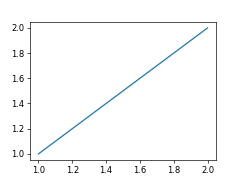
\includegraphics[width=0.92\textwidth]{figures/parameter_floor.png}
  \caption{Fine-tuned specialist success against parameter count, per
  subroutine, on held-out repositories. The dashed line is the 0.90
  reliability bar.}
  \label{fig:floor}
\end{figure}

\subsection{Fine-tuning, not scale, buys schema reliability}

\ftVsBaseNarrative{}

\begin{figure}[t]
  \centering
  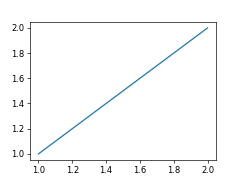
\includegraphics[width=0.85\textwidth]{figures/ft_vs_base.png}
  \caption{Mean success across subroutines for fine-tuned specialists versus
  base instruct models at identical sizes, prompts, and retry budgets.}
  \label{fig:ftbase}
\end{figure}

\subsection{Where rules suffice}

\rulesSufficeNarrative{}

\subsection{Cost per successful call}
\label{sec:cost}

\costNarrative{}

\subsection{Failure analysis}

\failureNarrative{}

% ---------------------------------------------------------------- 10
\section{MCP Deployment Architecture}

The research pipeline is deliberately orchestrator-free, routing is
deterministic and no master model is needed to produce any number above. For
deployment we expose the specialists to frontier coding agents through MCP.
The server presents a few coarse tools rather than dozens of micro-tools.
\texttt{slm\_run\_specialist\_task} is the generic entry point, with
convenience aliases such as \texttt{slm\_repair\_action},
\texttt{slm\_normalize\_path}, and \texttt{slm\_localize\_failure}. Behind
the tool boundary one pipeline runs every call. Render the input, invoke the
specialist backend, parse against the closed schema, check the deployment
guard, retry once on schema failure, and fall back to the rules solver if the
specialist cannot produce a guard-passing output. The orchestrator sees only
verified structured results. Backends are pluggable. The reference backend
runs rules only and needs no GPU, a local backend serves the fine-tuned
checkpoints, and the same interface admits a remote endpoint. A working
stdio JSON-RPC server implementing initialize, tools/list, and tools/call
ships in the repository with protocol tests.

% ---------------------------------------------------------------- 11
\section{Limitations}

Five repositories from the well-maintained Python ecosystem are not the
universe of code, and Python's regular syntax makes several rules baselines
unusually strong, so floors may differ in other languages. The two held-out
phrasing template banks were written by the same authors as the training
banks, which bounds but does not eliminate stylistic leakage. The grid mixes
two model families. Tasks are evaluated as isolated calls, not inside a live
agent loop, so compounding effects across calls are out of scope here, though
the previous study measured a full loop for one role. Synthetic tracebacks,
while built from real frames, are cleaner than production failures. The cost
model charges GPU seconds at rental price and omits engineering time.

% ---------------------------------------------------------------- 12
\section{Future Work}

The natural next steps are per-size hyperparameter tuning (one schedule was
used for all cells), sub-100M encoder-style classifiers for the pure routing
tasks, quantized on-CPU deployment measurements for the 135M and 360M floors,
non-Python languages where rules baselines weaken, and an end-to-end agent
study where a frontier orchestrator delegates through the MCP server under
real workloads.

% ---------------------------------------------------------------- 13
\section{Conclusion}

\conclusionNarrative{}

\paragraph{Reproducibility.} Every dataset is regenerated deterministically
from pinned repository tags and seeds by committed code. Training and
evaluation artifacts, per-cell JSON results, the parameter-floor JSON, and
all figures are committed at \repo.

\bibliographystyle{plainnat}
\bibliography{refs}

\end{document}
